\documentclass[11pt]{article}

\usepackage[paper=letterpaper,
           marginparwidth=1in,
           hmargin={1.3in,.3in},
           vmargin={1in,1.5in},           
           includemp
           ]{geometry}
           
 \usepackage{longtable}
 \usepackage{graphicx}
 \usepackage{caption}
 \usepackage{placeins}
\usepackage{subcaption}
\usepackage[]{natbib}
\usepackage{latexsym,amsfonts,amssymb,amsmath,amsthm,mathrsfs}
\usepackage{bbm}
\usepackage{amsthm}
\newtheorem{definition}{Definition}
\usepackage{hyperref}
\usepackage{lscape}

\hypersetup{
    bookmarks=true,         % show bookmarks bar?
    unicode=false,          % non-Latin characters in Acrobat’s bookmarks
    pdftoolbar=true,        % show Acrobat’s toolbar?
    pdfmenubar=true,        % show Acrobat’s menu?
    pdffitwindow=false,     % window fit to page when opened
    pdfstartview={FitH},    % fits the width of the page to the window
    pdftitle={My title},    % title
    pdfauthor={Author},     % author
    pdfsubject={Subject},   % subject of the document
    pdfcreator={Creator},   % creator of the document
    pdfproducer={Producer}, % producer of the document
    pdfkeywords={keyword1} {key2} {key3}, % list of keywords
    pdfnewwindow=true,      % links in new window
    colorlinks=true,       % false: boxed links; true: colored links
    linkcolor=red,          % color of internal links (change box color with linkbordercolor)
    citecolor=black,        % color of links to bibliography
    filecolor=magenta,      % color of file links
    urlcolor=blue           % color of external links
}

\title{Dynamic matching procedures for causal inference in social networks}

\providecommand{\keywords}[1]{\textbf{\textit{Keywords ---}} #1}


\author{{\textsc{Imanol Arrieta Ibarra}} \\
%EndAName
 \and {\textsc{Thomas Palomares}} \\
%EndAName
}



\begin{document}

\maketitle


\begin{abstract}
We design a matching mechanism for evolving networks. We simulate a graph model for which nodes form new edges over time. We compute for each node an output, happiness , depending notably on the happiness of a node's friends ( which could also be obesity, loneliness or any other behavior that may spread through a social network). We focus on extracting the treatment effect of a node making a friend who is happier than she is. We explain why this is the best we can do when matching based on edge formation. Furthermore, from the three matching mechanisms we tried, not one was able to recover the true treatment effect. This exposes some of the comebacks of using matching procedures in observational studies. 

\end{abstract}

\newpage

\section{Introduction}




\section{Motivation and Background}

Is obesity contagious? Can happiness spread through social networks? Is loneliness viral? Does befriending happy people makes us happier or do we tend to be friends of people with similar happiness as ours?. These questions have generated big controversy after \cite{christakis2007spread} affirmed that this phenomena diffuse thorough social networks similar to how a disease would.They deal on  the inquest of differentiating between homophily and influence based contagion abundant in causal inference literature. Fowler and Christakis intended to address this when investigating the effect of having obese friends to one’s obesity in \citep{christakis2007spread} and then on one’s happiness on. Also, \citep{cacioppo2009alone} studied how “lonely people tend to receive fewer friendship nominations, but they also tend to name fewer people as friends”. However \citep{shalizi2011homophily} argued that the results from all these studies were inconclusive due to possible confounders when working with observational studies. Furthermore, \citep{cohen2008detecting} later detected implausible social network effects in acne, height, and headaches using the same methodology and dataset as Fowler and Christakis . \\

Although distinguishing between homophily and influence based contagion in a static network was proven to be impossible, \cite{aral2009distinguishing} argued that by using propensity score matching on an evolving network, they were able to get the true influence effect ( or at least a bound to homophily). They did so by computing the propensity of a friend on adopting a new platform called Yahoo Go.\\

However, most of the Network theory does not provide an understanding of the evolutionary dynamics of observed processes. Indeed, most studies observe edges and friendships as one-time snapshots, while these relations are actually evolving over time. Based on \cite{aral2009distinguishing}, we wanted to investigate if matching methods could possibly capture the effect of a friends happiness on ours.\\

The goal of our project is to build a matching procedure on evolving networks that could be used to elicit the effect of an alter’s behavior on the ego’s behavior ( happiness, loneliness, obesity). We planned to test this procedure on simulated data to make it adaptable to the Framingham dataset. For that purpose we first designed a graph generating model which takes place in different stages. At each stage, friendships are created and we recompute the happiness of all the nodes. We then tried three matching procedures: propensity score matching (PSM), greedy matching with caliper using propensity scores (GPS), and greedy matching on the edge’s endpoints (GEP).\\

We also computed the true effect by running simulations and computing the average treatment effect on the treated. Unfortunately not one of the matching procedures we tried provided us with an unbiased estimate with low variance. PSM’s variance made it un-meaningful, while GPS and GEP had high bias.\\

In section \ref{Network Creation Model}, we present the graph creation algorithm and how happiness was computed. Section \ref{Treatment Effect} defines the effect we are trying to elicit. Section \ref{Matching Mechanisms} describes the matching mechanisms we tried. Section \ref{Results} show the results, possible explanations of why we were not able to identify the treatment effects and conclusions.\\

\section{Network Creation Model}
\label{Network Creation Model}

\subsection{Simulated model}

Similar to \cite{shalizi2011homophily}, we developed a network creation model which is ran in two stages. In a first stage, we allow each node to nominate a friend. In the second stage we compute the happiness of all the nodes.

\subsection{Graph simulation}

We first construct a one-regular directed graph with N nodes, endowed with observable characteristics X and unobserved characteristics Z. For parsimony, we defined X and Z as scalars, but a more complete model would have considered them as vectors. When populating the nodes with X and Z values we defined these as uniform random variables in [-1,1]. We could think that X represents a node ability to pay for her expenses and Z how she feels about Star Wars ( it is well known that Star Wars fans are a happier crowd who also tend to group together). \\

Initially we assign one friend to each node based on their similarity, then , at each step in time, we choose $30\%$ of nodes to which we'll assign a new friend. Every time we assign a friend to a node i, we apply the following procedure:

\begin{enumerate}
\item For each node we create a set of candidates based in probability: $\text{logit}^{-1} \left(-3||(X_i,Z_i)-(X_j,Z_j)||\right)$.
\item Then from the set of candidates, we pick one at random to be the nominated friend.
\end{enumerate}

Figure \ref{fig:graph} shows an example of how a random friend graph looks like after one step in which new friendships are formed.

\begin{figure}[h]
\centering
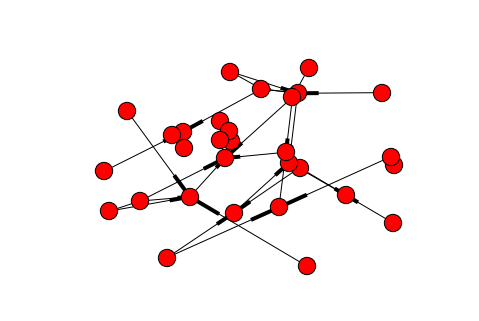
\includegraphics[scale=.3]{example_graph.png}
\caption{A random example of the friend's graph }
\label{fig:graph}
\end{figure}

\FloatBarrier
\subsection{Computing Happiness}

At step 0, for each node, we compute happiness according to their observable and unobservable characteristics. In particular we use the formula:
$$H_{i,t} = w_0 +w_1 X_i+w_2 Z_i + \epsilon_i$$

 After the edges have been added, we compute the happiness according to the following equation:
$$H_{i,t} = w_0 +w_1 H_{i,t-1} + w_2 \frac{1}{|N(i)|} \sum\limits H_{j,t-1} + w_3 X_{i} + w_4 Z_{i} + \epsilon $$

When the happiness is updated for every node in the network, we re update the set of friends candidate for each node.\\

In real life it is hard to believe that our happiness depends on our friends’ happiness on previous years. However we needed to make this assumption in order to keep the model as simple as possible. Otherwise we would have to compute a fixed point at every timestep ( assuming that such a fixed point exists). 


\section{Treatment Effect}
\label{Treatment Effect}
Under perfect circumstances we would be interested in eliciting the effect of an alter’s happiness ( weight, loneliness, etc…) on the happiness of the ego. However, by limiting ourselves to matching mechanisms on edge formation, this effect is unidentifiable. The reason is because edge formation only provides information about the channel through which influence can flow. It says nothing about what kind of response this influence provoques. Since there are cases when an alter is happier than the ego and other cases when she is sadder, this effects would cancel out. The only case when we would be able to identify an effect would be when only one of the two directions has an effect on the ego. This is, imagine that the ego’s happiness is only influenced by happier friends, then we would be able to identify the effect. 

Now, we could compute the absolute effect which would provide us with a measurement of how influential friends are in certain behaviors. However we would lose the direction of the effect in this case. We would not know if only happy friends drive you happier or if only sad friends make you sadder. When taking policy decisions this is a crucial distinction. 

For the reasons presented in the previous paragraphs, we decided to define the treatment as the formation of an edge with an alter who is happier than the ego. This would allow us to identify both the magnitude and the direction of the effect, limiting ourselves to only one side of the effect. We could also compute the same for sadder alters but this is not necessary if irrelevant for policy decisions. 

\section{Matching mechanisms}
\label{Matching Mechanisms}
We tried three different matching mechanisms in order to recover the desired treatment effect: propensity score matching, greedy matching with caliper based on the propensity score and matching based on the similarity between the endpoints of two edges. Propensity score matching gave us a huge estimate which in terms of any real application would have been meaningless. Greedy matching provided a more stable, however biased, estimate. Finally, matching based on the endpoints returned a much more stable estimate of the treatment effect, but still a biased one. 

\subsection{Propensity Score Matching (PSM)}

We computed our first treatment estimate using propensity score matching according to the following equation:

$$\hat{\tau} = \sum\limits_i\sum\limits_j Y_{i,j}^{(1)}\frac{\mathbb{I}\{i \rightarrow j\}}{\hat{\mathbb{P}}(i\rightarrow j)} - \sum\limits_i\sum\limits_j Y_{i,j}^{(0)}\frac{\mathbb{I}\{i \rightarrow j\}}{\hat{\mathbb{P}}(i\rightarrow j)}$$

where:
$$Y_{i,j}^(k) = H_{i,t}-H{i,t-1}$$

We estimated the propensity scores using logistic regression with the response variable being the existence of an edge from i to j such that the j's happiness was bigger than i's. The only regressor was the observable variable. While this is a reasonable estimation of the probabilities, it is important to remember that the real probabilities were highly non-linear although they did had a logistic component based on the observable variable. However, the predictions we obtained were not very good at properly estimating the real probabilities. We realized this by simulating new data and testing it with the predictors. 

\subsection{Greedy Matching with Caliper based on Propensity Scores (GPS)}
For this method, we used the propensity scores computed when doing PSM and performed greedy matching on them. We separated the treatment examples from the untreated ones and shuffled the treatments. Then for each edge in the treatment group, we greedily choose the edge in the untreated group with the closest propensity score. We repeated this with replacement until all treatment edges had been matched. We then discarded any pair of edges whose difference of PS was smaller than the specified caliper ( 0.05 for our case). Finally we ran a linear regression with the change in happiness as the response variable and the treatment as the regressor. This provided an estimate for the average treatment effect on the treated.

\subsection{Greedy Matching on the edge's endpoints (GEP)}

There are several problems when matching with propensity scores. In general these are summarized quite well in …(Gary King). For our particular application, we encountered that matching on propensity could provide wrong estimates by the nature of the method. Figure … evidenciates one of these issues. On it , the left clique is matched to the right one. However, although an edge was formed on the left clique and none was formed on the right one, the estimate would be negative. This does not mean that the effect of adding a happier friend is negative. In part this has to do with our choice of computing an ego’s happiness based on the lagged happiness of her friends.\\

One way to solve this problem is to match the edges based on the endpoints. This makes comparisons between edges more robust but still presents difficulties regarding our choice of happiness depending on friends' lagged happiness. Unfortunately the only way to solve for this issue is to match on the whole ego network and this would be prohibitive in any real graph.


\section{Results and Limitations}
\label{Results}

The assumption that the current happiness depends only of the previous happiness of the person and of their friends is a clear limitation of the model. It is also a very useful assumption allowing us to easily compute the happiness without computing an expensive fixed point equilibrium at each step. It would be interesting as future work to correctly model this part of the model. Maybe by doing so many of the counter-intuitive results may be solved.

As explained above, none of the matching procedures provided us with a useful estimate. We will proceed by showing the results for the greedy matching mechanisms since the variance of the propensity score matching procedure only gave us gibberish.

We first wanted to observe if out process would identify small effects or no effects. For an effect of zero we were able to identify it and both of our matching procedures were centered in zero with small variance. This indicates that the power of our test is high. Figures \ref{fig:no_effect_gps} and \ref{fig:no_effect_gep} show this case. The expected value for the four distributions is close to zero.


\begin{figure}[h]
\centering
\begin{subfigure}{.5\textwidth}
  \centering
  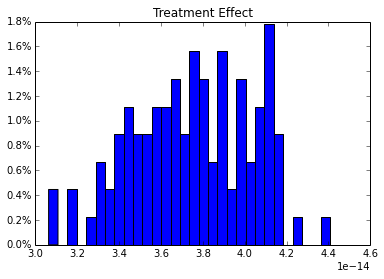
\includegraphics[width=.9\linewidth]{treatment_effect_no_influence_real.png}
  \caption{True treatment effect computed by simulations}
  \label{fig:sub1}
\end{subfigure}%
\begin{subfigure}{.5\textwidth}
  \centering
  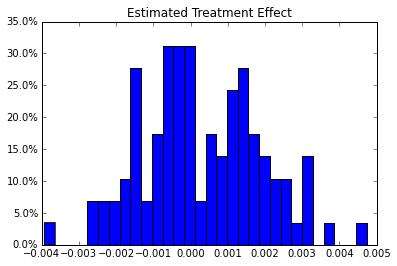
\includegraphics[width=.9\linewidth]{estimated_no_influence.png}
  \caption{Estimated effect}
  \label{fig:sub2}
\end{subfigure}
\caption{Coefficient estimation when there is no effect for greedy matching with caliper.}
\label{fig:no_effect_gps}
\end{figure}

\begin{figure}[h]
\centering
\begin{subfigure}{.5\textwidth}
  \centering
  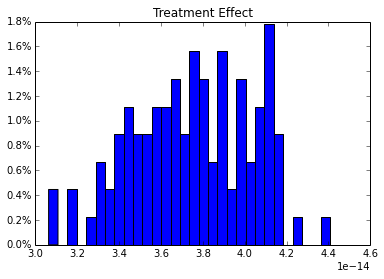
\includegraphics[width=.9\linewidth]{treatment_effect_no_influence_real.png}
  \caption{True treatment effect computed by simulations}
  \label{fig:sub1}
\end{subfigure}%
\begin{subfigure}{.5\textwidth}
  \centering
  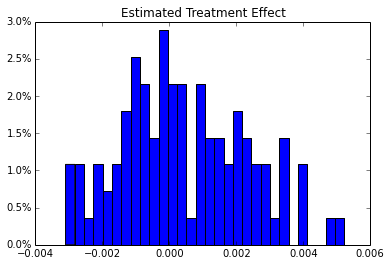
\includegraphics[width=.9\linewidth]{estimated_no_influence_gep.png}
  \caption{Estimated effect}
  \label{fig:sub2}
\end{subfigure}
\caption{Coefficient estimation when there is no effect for GPS.}
\label{fig:no_effect_gep}
\end{figure}

Then, we  wanted to observe if out process would identify small effects or almost zero effects. For an effect of 0.002 GPS was able to produce an unbiased estimate but the variance would not have allow us to reject the null hypothesis. GEP returns a biased estimator with low variance. Figures \ref{fig:small_effect_gps} and \ref{fig:small_effect_gep} show this case. 

\begin{figure}[h]
\centering
\begin{subfigure}{.5\textwidth}
  \centering
  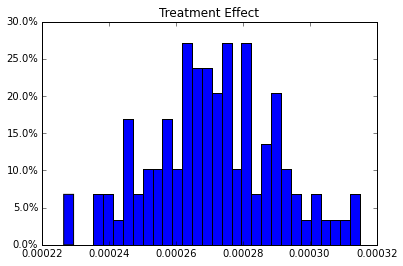
\includegraphics[width=.9\linewidth]{treatment_effect_no_influence.png}
  \caption{True treatment effect computed by simulations}
  \label{fig:sub1}
\end{subfigure}%
\begin{subfigure}{.5\textwidth}
  \centering
  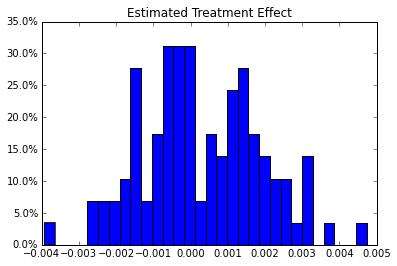
\includegraphics[width=.9\linewidth]{estimated_no_influence.png}
  \caption{Estimated effect}
  \label{fig:sub2}
\end{subfigure}
\caption{Coefficient estimation when there is no effect for GEP.}
\label{fig:small_effect_gps}
\end{figure}

\begin{figure}[h]
\centering
\begin{subfigure}{.5\textwidth}
  \centering
  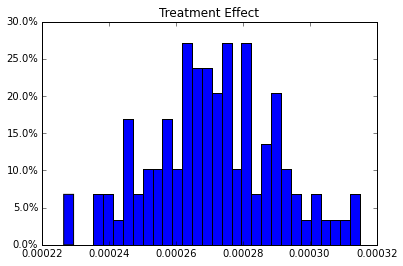
\includegraphics[width=.9\linewidth]{treatment_effect_no_influence.png}
  \caption{True treatment effect computed by simulations}
  \label{fig:sub1}
\end{subfigure}%
\begin{subfigure}{.5\textwidth}
  \centering
  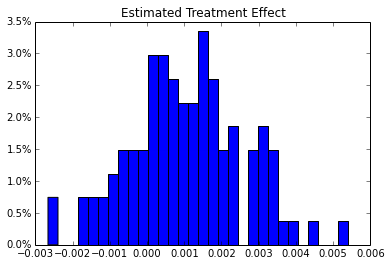
\includegraphics[width=.9\linewidth]{estimated_small_effect_gep.png}
  \caption{Estimated effect}
  \label{fig:sub2}
\end{subfigure}
\caption{Coefficient estimation when there is an effect of 0.002 for GEP.}
\label{fig:small_effect_gep}
\end{figure}

\FloatBarrier

Finally , we  tried to estimate a large effect. For an effect of 0.35 both GPS and GEP provided a result close to 0.25 which means that these estimators are biased.   Figures \ref{fig:large_effect_gps} and \ref{fig:large_effect_gep} show this case. 

\begin{figure}[h]
\centering
\begin{subfigure}{.5\textwidth}
  \centering
  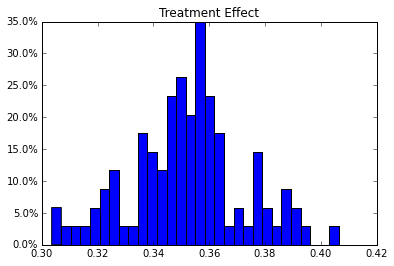
\includegraphics[width=.9\linewidth]{treatment_effect.png}
  \caption{True treatment effect computed by simulations}
  \label{fig:sub1}
\end{subfigure}%
\begin{subfigure}{.5\textwidth}
  \centering
  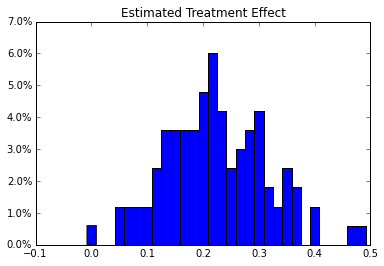
\includegraphics[width=.9\linewidth]{estimated_treatment_effect.png}
  \caption{Estimated effect}
  \label{fig:sub2}
\end{subfigure}
\caption{Coefficient estimation when there is no effect for GEP.}
\label{fig:large_effect_gps}
\end{figure}

\begin{figure}[h]
\centering
\begin{subfigure}{.5\textwidth}
  \centering
  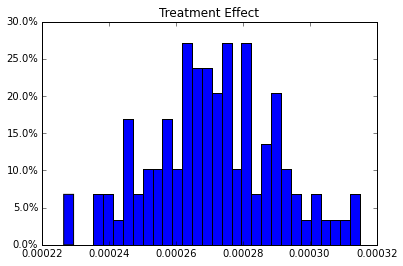
\includegraphics[width=.9\linewidth]{treatment_effect_no_influence.png}
  \caption{True treatment effect computed by simulations}
  \label{fig:sub1}
\end{subfigure}%
\begin{subfigure}{.5\textwidth}
  \centering
  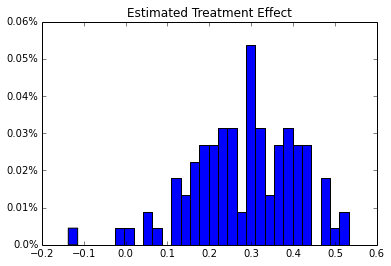
\includegraphics[width=.9\linewidth]{estimated_large_effect_gep.png}
  \caption{Estimated effect}
  \label{fig:sub2}
\end{subfigure}
\caption{Coefficient estimation when there is an effect of 0.002 for GEP.}
\label{fig:large_effect_gep}
\end{figure}

\FloatBarrier
\section{Conclusions and future work}
Throughout this project we found several issues regarding the estimation of causal effects on observational studies. We showed that even for very simplistic models, identifying an influence effect is very complicated. It is in particular difficult to isolate and measure the influence of one single effect (here befriending a happier friend) and distinguishing phenomena occurring simultaneously, such as the effect of the creation of an edge in itself or the influence of an happier friend on a node. This puts some doubts on Aral et all’s findings as well as on similar methods that haven’t been confirmed on simulated or known datasets. \\

For future work, it would be interesting to perform a deeper analysis on this model to understand what is causing the estimators to be biased. If this is overcome, many relevant questions may be further analyzed: how to generalize this matching method for multiple time-steps?. Moreover, it would also be exciting to add a tie breaking component and to study the influence of dropping a friend.

Finally, testing \citep{aral2009distinguishing} algorithm on a simulated model and observing if known influence can be revealed by their method would be an interesting lead to understand better which phenomena are at stake in this model.
	

\newpage
\bibliographystyle{chicago}
\bibliography{biblio}
\nocite{*}

\end{document}